\chapter{OpenStreetMap}
\label{cap:OpenStreetMap}
In questo capitolo si illustra brevemete il progetto OpenStreetMap, vengono sollevate alcune questioni etiche nella scelta di un map-provider e infine si espongono i motivi tecnici che hanno portato a scegliere OSM come map-provider per l'applicazione sviluppata nell'ambito di questa tesi.
\section{Cos'è OpenStreetMap ?}
OpenStreetMap (OSM) è \textbf {un progetto cartografico collaborativo, nato per creare una mappa mondiale gratuita e libera}. Gli utenti iscritti possono visualizzare, aggiungere e modificare in ogni momento la mappa, secondo un approccio analogo a quello di Wikipedia. I dati infatti sono distribuiti sotto la licenza ODbl\cite{LICENZA_OSM}: \textit{"Sei libero di copiare, distribuire, trasmettere e adattare i nostri dati, finchè lo attribuisci a OpenStreetMap e ai suoi contributori. Se alteri o ti basi sui nostri dati, puoi distribuire il risultato sotto la stessa licenza [...]"}.\\
\begin{figure}[H]
	\centering
	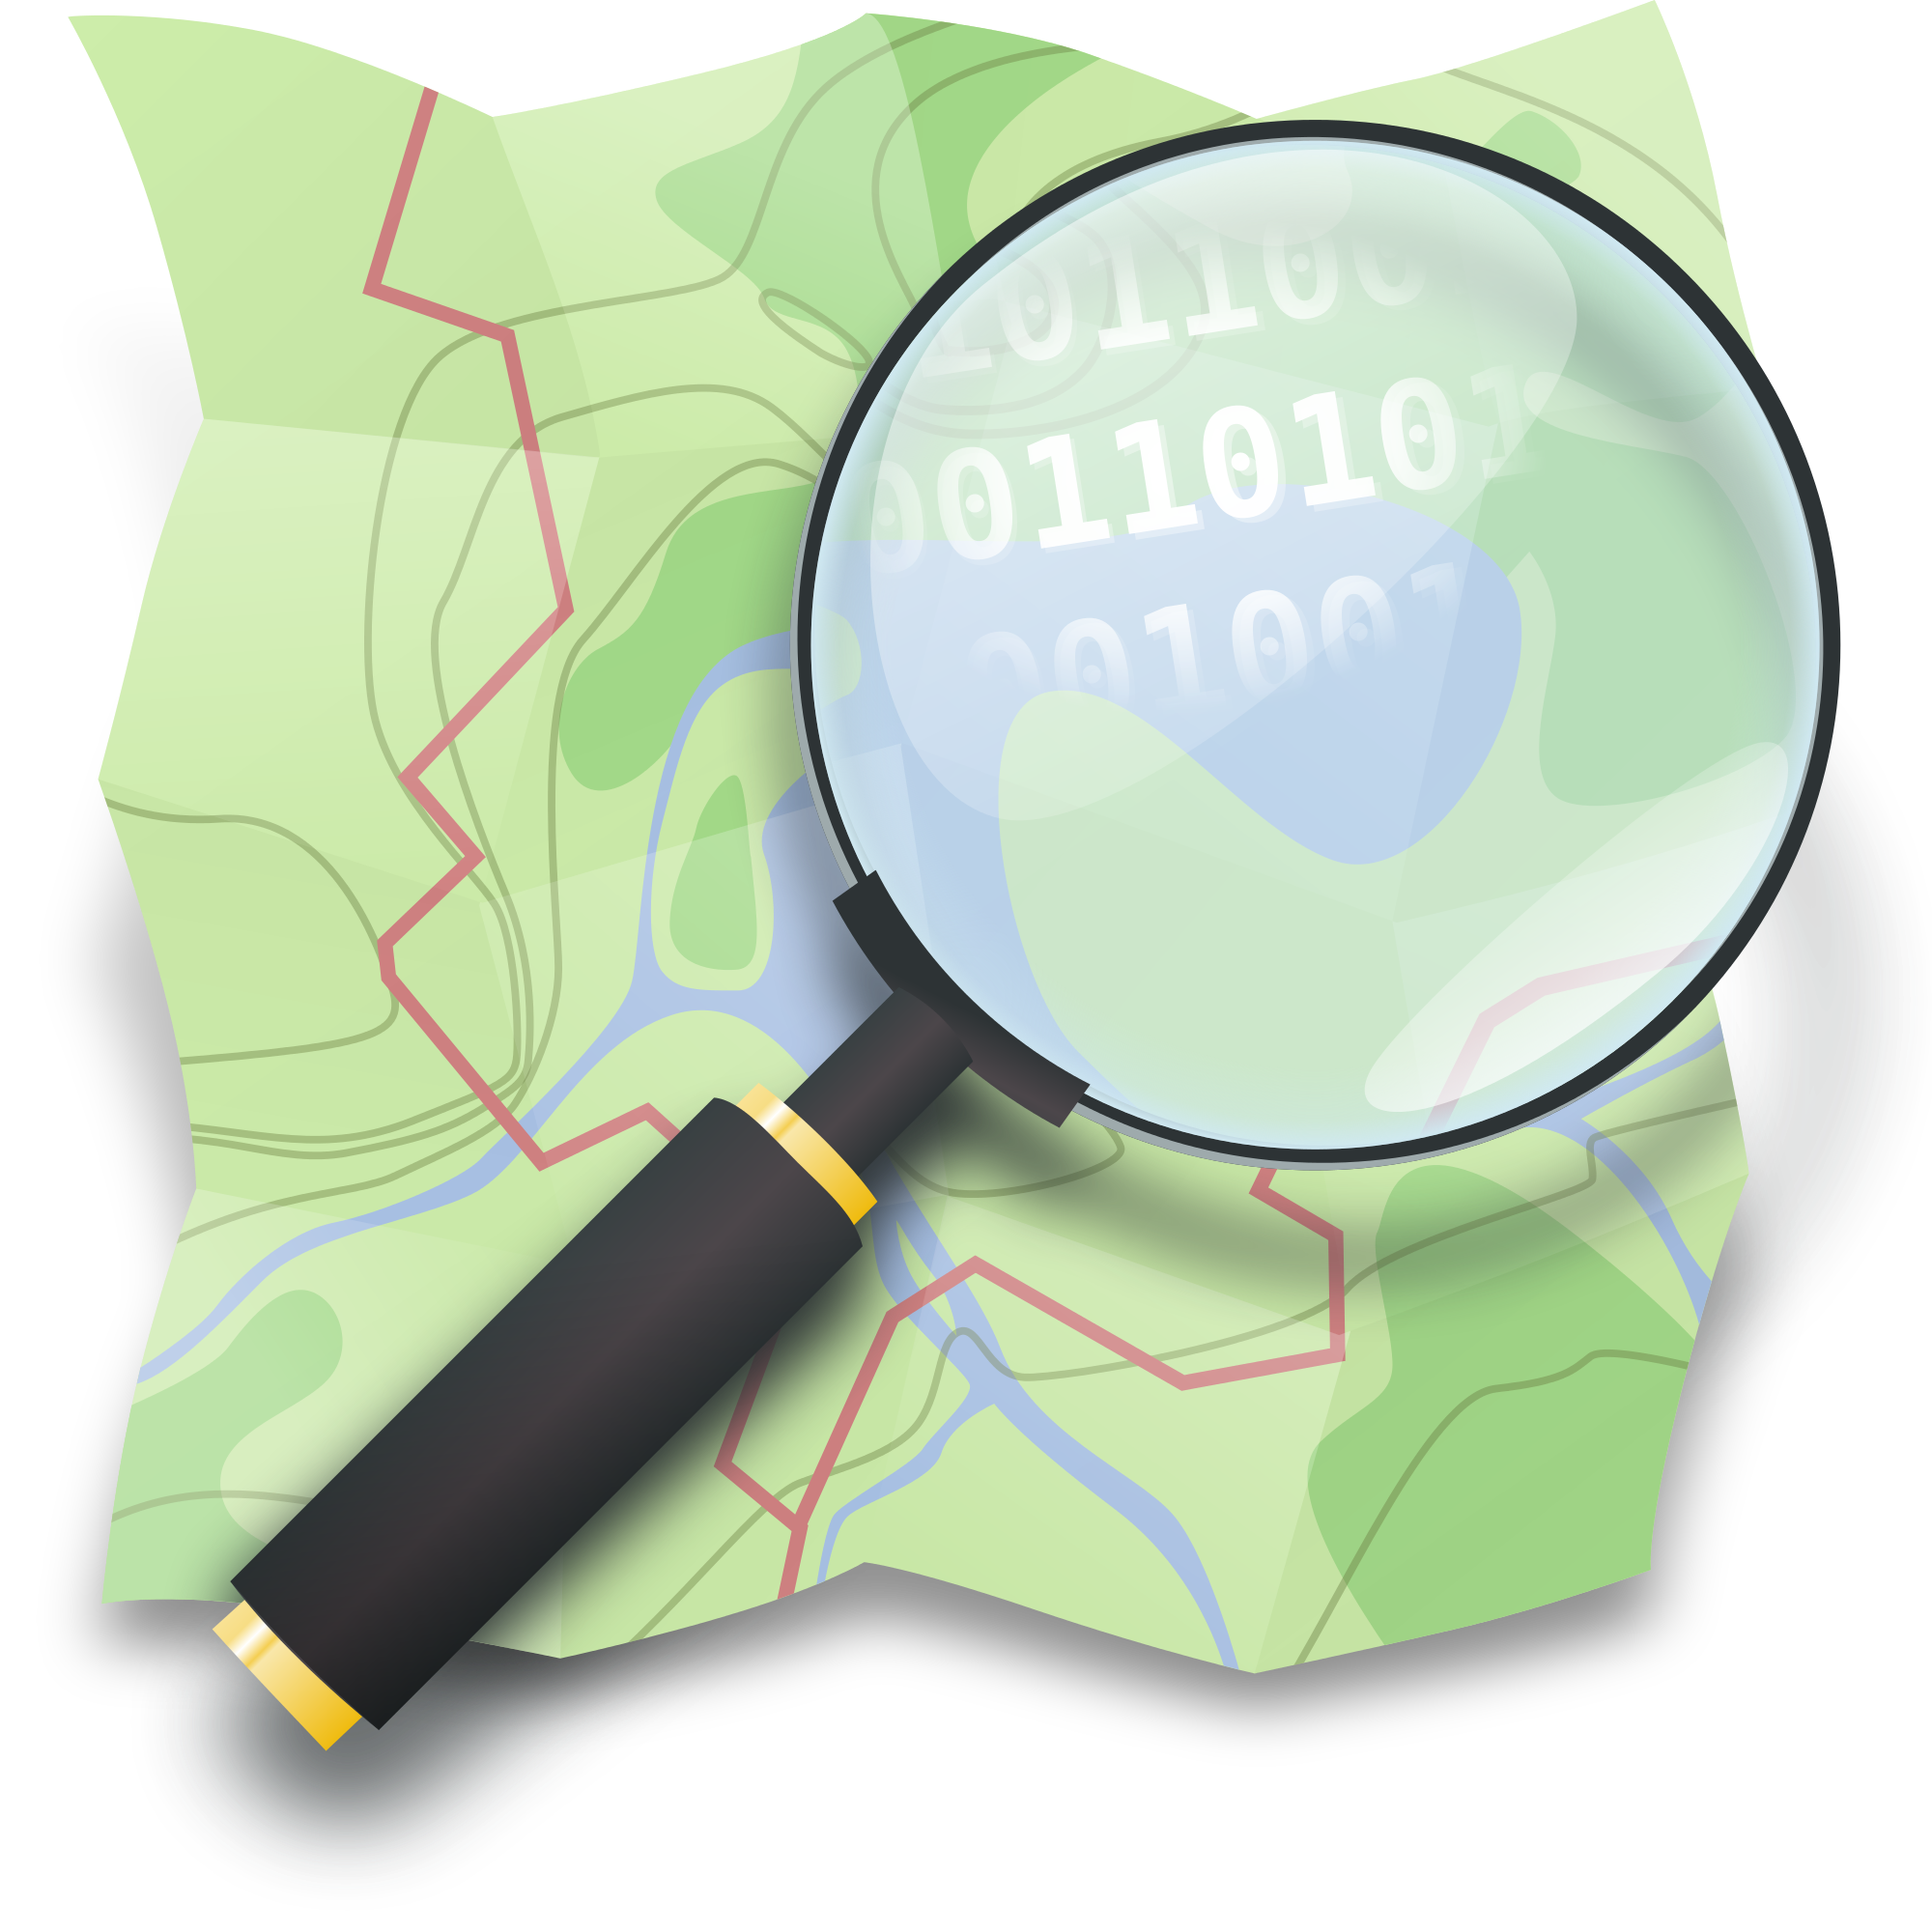
\includegraphics[scale=0.1]{OpenStreetMap/logo.png}
	\caption{Il logo di OpenStreetMap}
	\label{fig:logo_OSM}
\end{figure}
Si potrebbe erroneamente pensare che l'esistenza di una mappa gratuita non sia una novità; in realtà  i dati geografici \cite{MAPPE_LIBERE}, nella gran parte del mondo (Italia ed Europa incluse), non sono gratuiti. In linea di massima l'onere della realizzazione di mappe è delegata ad agenzie nazionali che poi le rivendono a privati o aziende e ne ricavano finanziamenti. Gli Stati Uniti d'America sono l'unica eccezione macroscopica: qui, infatti, le leggi sul copyright delle agenzie nazionali rendono questi dati di pubblico dominio.\\
In altre parole se si vive in uno di questi paesi, si pagano le tasse perché vengano realizzate le mappe e si paga nuovamente per avere copie di esse o meglio "fotocopie". Di fatto si tratta di vere e proprie fotocopie poiché non possono essere modificate, sebbene spesso le mappe contengano errori intenzionali (chiamati in gergo easter eggs). Si tratta solitamente di strade inesistenti o mancanti, oppure indicazione di edifici che in realtà non esistono. Se si tenta di realizzare una mappa partendo da questi dati, le ditte od enti che le hanno realizzate potranno dire di avervi beccato semplicemente controllando se sono presenti i loro errori.\\
La comunità di OSM è in forte crescita: dal 2004, anno in cui nasce da un'idea di Steve Coast ,ad oggi, il numero di utenti iscritti e i loro contributi sono cresciuti anno dopo anno, come illustrato in Figura 1.2 .
\begin{figure}[H]
	\centering
	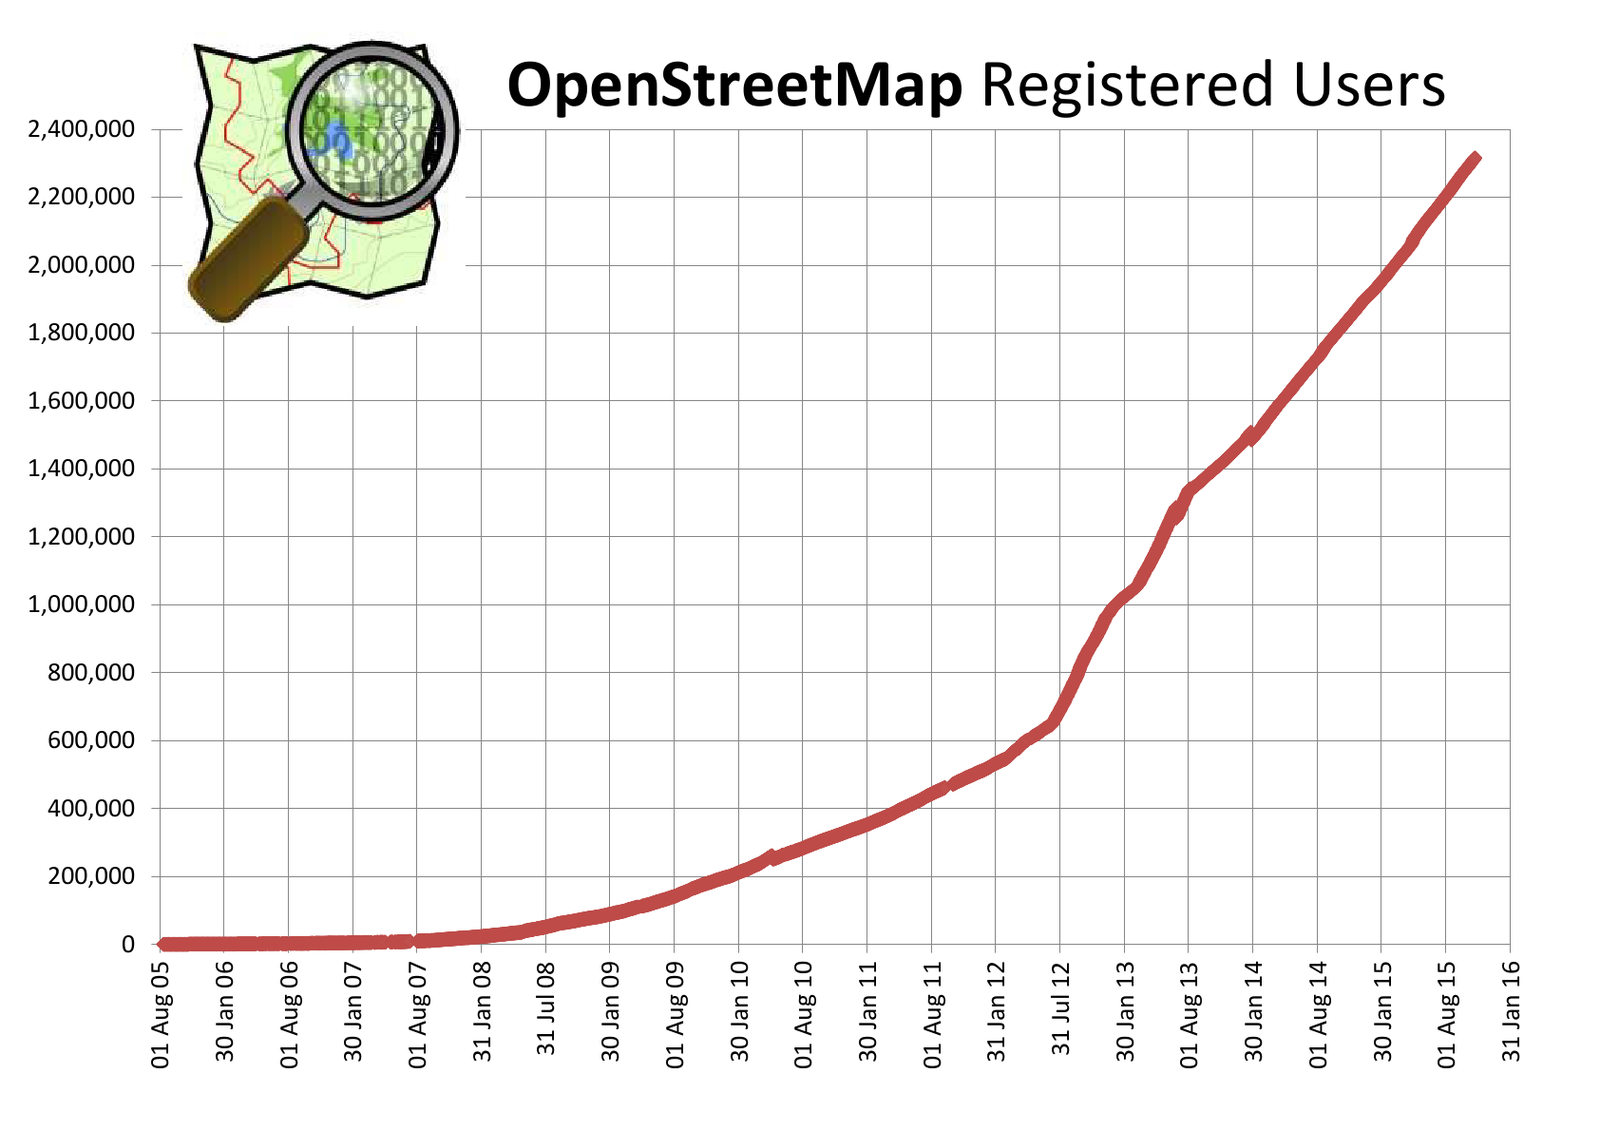
\includegraphics[scale=0.5]{OpenStreetMap/utenti.png}
	\caption{Scala lineare di utenti iscritti ad OpenStreetMap}
	\label{fig:utenti_OSM}
\end{figure}
Nel prossimo paragrafo si illustreranno meglio i motivi dell'esistenza di un progetto come OSM.


\newpage 
\section{Perchè il mondo ha bisogno di OSM} 

Finora quello di OSM sembrerebbe un altro progetto di nobile causa ma fine a se stesso. Per comprendere meglio la sua importanza bisogna fare un passo indietro nella storia e tornare nel 1800 \cite{WHYNEED} .\\
In quel periodo uno dei tanti problemi era costituito dal tempo, non in termini di tempo a disposizione, ma di che ora fosse. Gli orologi esistevano già, ma ogni città aveva il suo "tempo locale". Viene da sé come anche prendere un banale appuntamento con l'amico del paese vicino, comportasse una grande difficoltà. Successivamente l'adozione di uno standard comune ha reso il tempo \textbf{universale, libero e di tutti}.
L'equivalente attuale del dilemma del tempo è la posizione geografica, e diversi soggetti stanno cercando di diventarne il riferimento assoluto (Google spende un miliardo di dollari l'anno per mantenere le proprie mappe). 
Dunque perché il mondo ha bisongo di OSM? La risposta è semplice, perché in una società nessuna azienda dovrebbe avere il monopolio su qualcosa. I luoghi sono un bene comune, e dando ad una o poche entità questo potere gli viene dato non solo il potere di dirti la tua posizione, ma anche di poterla manipolare.
Ci sono tre aspetti da analizzare:
\begin{itemize}
\item Cosa viene visualizzato
\item Dove dovresti andare
\item Privacy personale\\
\end{itemize} 

\textbf{Cosa viene visualizzato:} Chi decide cosa debba essere visualizzato su una mappa di Google? Ovviamente Google. Se pensiamo ad un servizio pubblico, questo deve essere il più imparziale e trasparente possibile, come potrebbe esserlo se utilizza un mappa di Google?.\\
Il punto è, nel momento in cui si sceglie un provider di mappe, gli viene dato il potere di decidere quali siano gli elementi a cui dare risalto, o quali non debbano essere proprio mostrati.\\\\
\textbf{Dove dovresti andare:} La seconda questione riguarda il posizionamento. Chi decide cosa sia più vicino a me? Ancora una volta la risposta è banale. Non è un caso che scrivendo su Google Maps la parola \textit{"colazione"} vengano mostrate le grandi catene come McDonald's piuttosto che il bar sotto casa.\\
Nell'immagine successiva viene mostrato uno screenshot della ricerca \textit{"colazione"} effettuata su Google Maps all'interno della biblioteca di scienze umane dell'universita dell'Aquila. 

\begin{figure}[H]
	\centering
	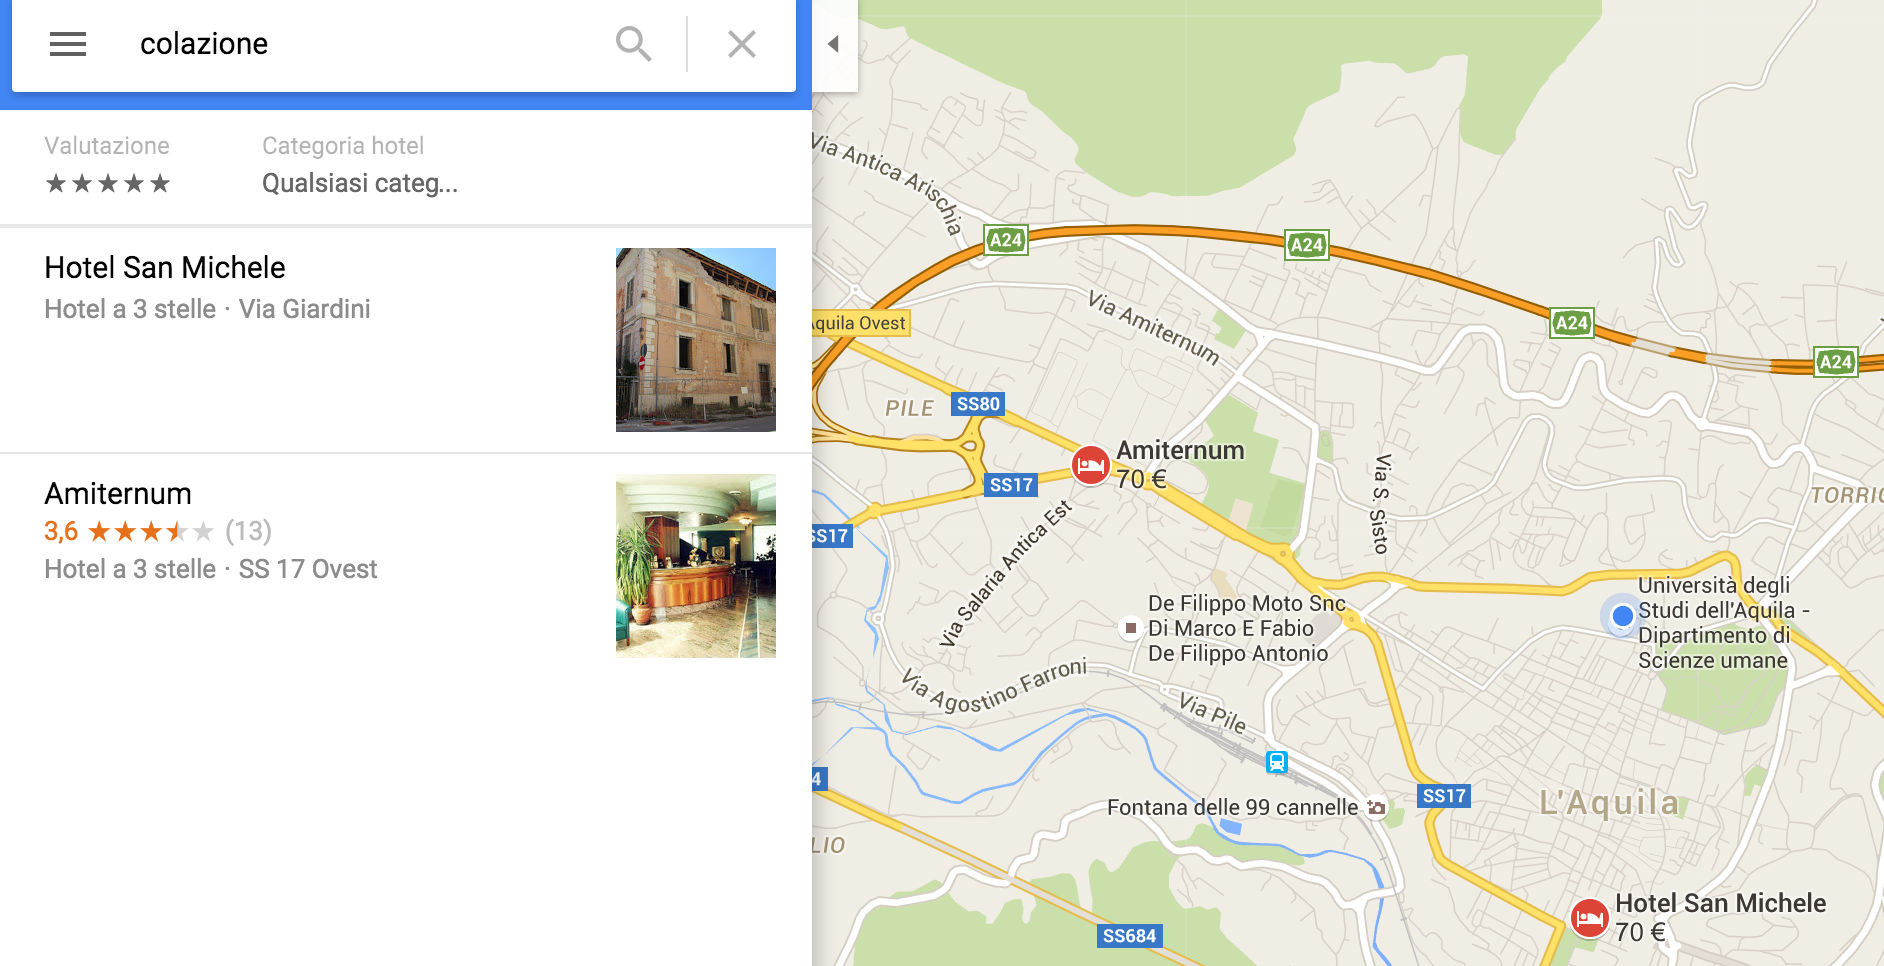
\includegraphics[scale=0.4]{OpenStreetMap/colazione.png}
	\caption{Risultato ricerca "colazione"}
	\label{fig:Ricerca_colazione}
\end{figure}

Come possiano notare vengono mostrati soltanto due hotel locali, che probabilmente hanno pagato il provider, nonostante ci sia un piccolo bar appena fuori la struttura.\\\\
\textbf{Privacy personale:} L'ultima questione riguarda la privacy. Sia Google che Apple raccolgono una quantita smisurata di informazioni sulla posizione degli utenti che utilizzano le loro API. E’ evidente che non si possono ignorare le implicazioni sociali che comporta la disponibilità di così tanti dati in mano ad una singola azienda, indipendentemente da quanto si dichiari benevola.  Aziende come Foursquare utilizzano il mezzo della “gamification” per coprire quello che di fatto è un’opera di acquisizione di dati, e anche Google è entrata nella partita della “gamification” con \textit{Ingress}, un gioco che sovrappone un mondo virtuale a quello reale e porta gli utenti a raccogliere foto e informazioni stradali con l’obiettivo di combattere, o favorire, un’invasione aliena.



\newpage
\section{OpenStreetMap vs Google Maps}
Tralasciando le questioni etiche e al fine della realizzazione dell'applicazione, sono stati analizzati i seguenti topic per la scelta del map-provider:
\begin{itemize}
\item Accuratezza
\item Costo e Download
\item Scalabilità\\
\end{itemize} 

\textbf{Accuratezza:} Poiché le mappe fornite da OSM sono il frutto di lavori "amatoriali", si è indotti a pensare che queste non rispecchino la realtà. Come in ogni progetto in stile wiki, non c'è alcuna garanzia riguardo l'accuratezza dei dati. C'è da dire, però, che quasi nessuna mappa "commerciale" dà alcuna garanzia di accuratezza. In fondo, gli errori intenzionali, sono per l'appunto, errori. \cite{ACCURATEZZA_MAPPE} \\
L'essenza stessa dei processi in stile wiki è che gli utenti stessi, tutti gli utenti, hanno un ruolo nell'accuratezza dei contenuti. Se qualcuno dovesse inserire dati errati, per errore o con intenzione, tutti gli altri possono accorgersene e correggere l'errore o semplicemente eliminarlo. La presenza di una larghissima maggioranza di utenti benintenzionati garantisce che gli errori restino entro un limite accettabile.\\
L'esperienza degli altri progetti basati su wiki ci insegna, comunque, quanto sia agevole raccogliere dati di buona/ottima qualità e quanto, invece, possa essere complicato scovare gli inevitabili errori.
Attualmente non sono stati realizzati processi o meccanismi che rendano semplice questo genere di controllo, tuttavia una comunità attiva come quella di OSM garantisce un controllo qualità sufficiente.\\
La domanda che dobbiamo porci è chi meglio di noi conosce il quartiere dove abitiamo? O la strada che percorriamo tutti i giorni o il parco dove portiamo il nostro animale a passeggiare? La risposta è \textbf{NOI}. Ed è proprio questo sottile concetto a fare la differenza tra una mappa OSM e una mappa proprietaria.\\
Utilizzando uno dei tanti "map-compare" sulla rete possiamo fare degli esempi concreti. Nella Figura 1.4 abbiamo una duplice visualizzazione dell'area universitaria di Coppito (L'Aquila): a sinistra vediamo la mappa ottenuta tramite dati OSM mentre a destra la stessa mappa fornita da Google.

\begin{figure}[H]
	\centering
	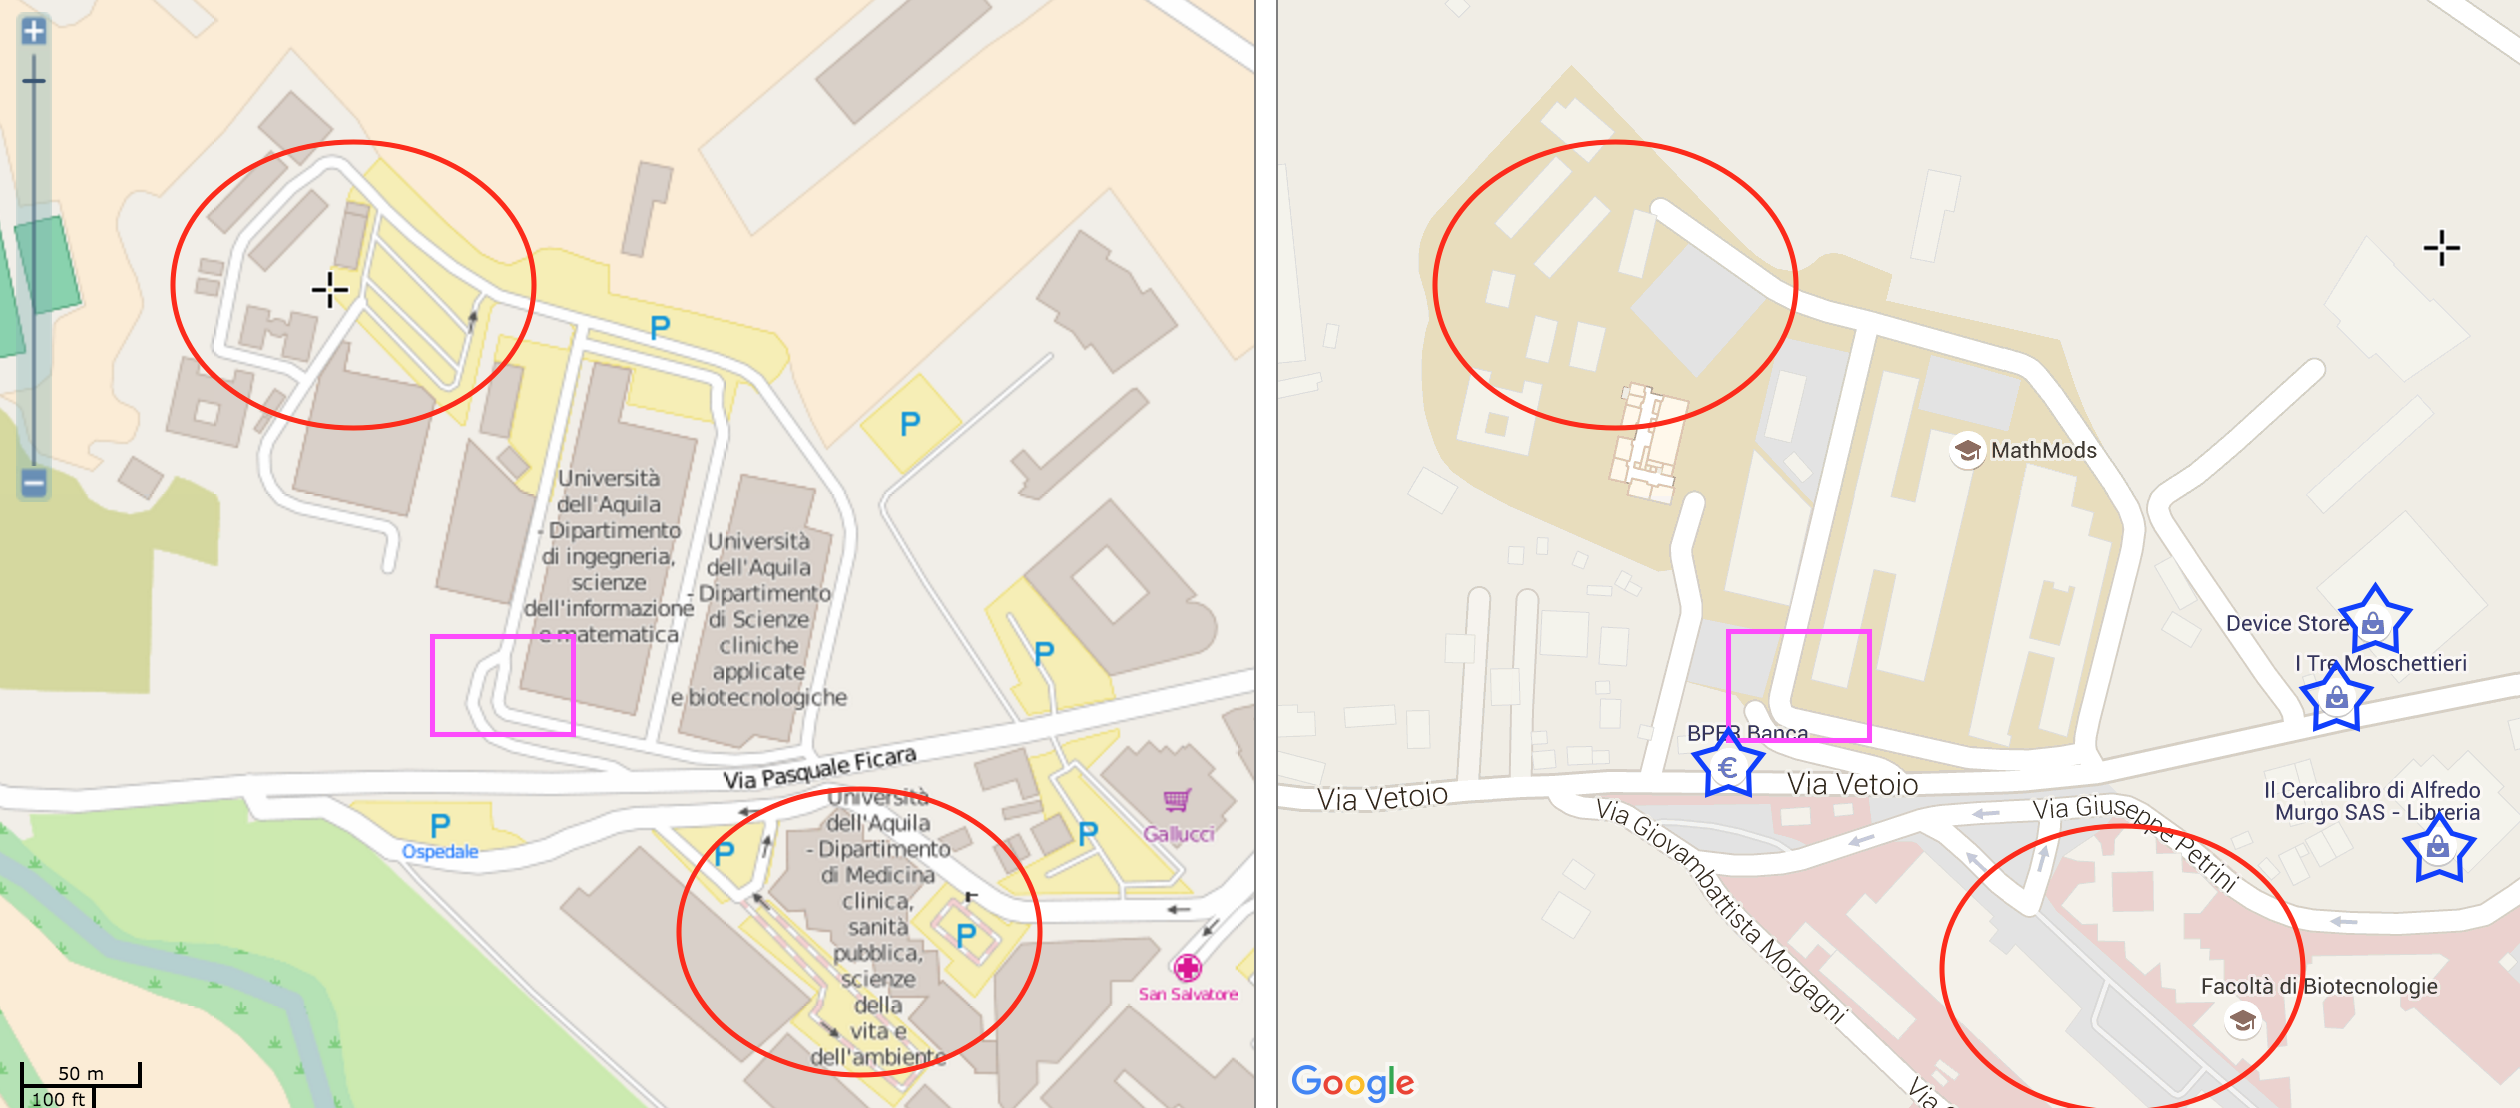
\includegraphics[scale=0.3]{OpenStreetMap/map_compare_coppito.png}
	\caption{Polo universitario di Coppito-L'Aquila}
	\label{fig:Compare_Coppito}
\end{figure}

Soffermiamoci quindi soltanto sulle porzioni di mappa racchiuse nelle diverse figure geometriche:

\begin{itemize}
\item \textbf{Cerchi rossi:} notiamo come nella mappa di Google siano assenti diverse strade interne alla struttura che collegano i diversi edifici tra di loro; questi sono percorribili da un veicolo d'emergenza o più semplicemente un'autovettura.
\item \textbf{Rettangolo viola:} Presenza di un errore (possibile easter eggs) da parte di Google: la strada non si interrompe in quel modo
\item \textbf{Stelle blu:} Presenti solo nella mappa di Google, indicano tutte attività commerciali, sarà un caso?
\end{itemize} 

Infine osservando la mappa fornita da Google non si percepisce di avere davanti una grande struttura universitaria, mentre sulla mappa OSM sono indicati perfino i nomi dei dipartimenti presenti nei diversi edifici. \newpage

\textbf{Costo e download:} Volendo realizzare un'applicazione per dispositivi mobili completamente gratuita, priva di pubblicità o di qualsiasi atra forma di lucro, di questo fattore non si può non tenere conto.
Per quanto riguarda Google, l'API javascript è gratis fino ad un massimo di venticinquemila richieste giornaliere per novanta giorni consecutivi. Superata questa soglia si ha un costo di \$ 0,50 ogni mille richieste \cite{GOOGLE_PLAN}. \\
Oltre al costo vengono applicate le seguenti restrizioni:

\begin{itemize}
\item \textbf{Area limitata:} è possibile scaricare una porzione di mappa la cui dimensione massima non superi i centoventimila chilometri quadrati              \cite{GOOGLE_OFFLINE}.
\item \textbf{Scadenza:} le mappe saranno disponibili in assenza di rete per un totale di 30 giorni, dopodiché si dovrà effettuare l'accesso alla rete.
\end{itemize}

Per quanto riguarda OSM, essendo un progetto open-data, non vi è alcuna restrizione. Infatti, è possibile scaricare l'intera mappa del mondo o porzioni di essa in totale libertà e conservarle a tempo indeterminato \cite{LINK_PLANET}.
\newpage

\textbf{Scalabilità:} Quest'ultimo topic ha segnato di fatto il punto decisivo per la scelta di OSM come map-provider. L'associazione no-profit HOT (Humanitarian Openstreetmap Team), ha lo scopo di fornire un valido supporto sul campo al mapping di aree colpite da disastri ambientali e non.\\
Nel sito ufficiale si possono visualizzare i rapporti delle principali emergenze a cui l'associazione ha partecipato \cite{HOT_PROJECT} , consideriamo quindi il terremoto di Haiti.\\
Il 12 gennaio 2010 un violento terremoto di magnitudo 7.0 Mw (quello che colpi L'Aquila nel 2009 fu di 6.3 Mw) con epicentro localizzato a circa 25 chilometri in direzione ovest-sud-ovest della città di Port-au-Prince, capitale dello Stato caraibico di Haiti, colpì tutta l'area circostante.\\
Il numero di vittime è stato stimato al 24 febbraio 2010 in 222.517. Secondo la Croce Rossa Internazionale e l'ONU, il terremoto avrebbe coinvolto più di 3 milioni di persone \cite{WIKI_HAITI}.\\ Sei ore dopo il disastro la mappa disponibile di Port-au-Prince era la seguente:

\begin{figure}[H]
	\centering
	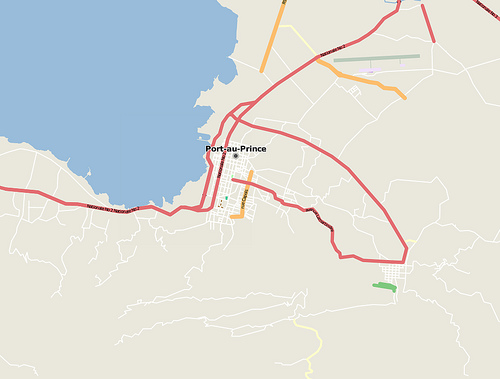
\includegraphics[scale=0.6]{OpenStreetMap/haiti_prima.jpg}
	\caption{Mappa OSM di Pourt-au-Prince 6 ore dopo il terremoto del 2010}
	\label{fig: haiti_day0}
\end{figure}
\newpage
Nelle ore successive, numerose aziende di geo-data (Geo-eye, Google, Yahooo...) resero pubbliche le proprie immagini satellitari, in modo tale che i volontari potessero mappare l'area colpita dal proprio pc in qualsiasi parte del mondo. \\
Quello che avvenne fu qualcosa di straordinario, come disse Jeffery Johnson \textit{"What we did in Haiti changed disaster response forever"}. \\
Il contributo di più di seicento volontari portò ad avere dopo appena 48h dal disastro la seguente mappa:

 \begin{figure}[H]
	\centering
	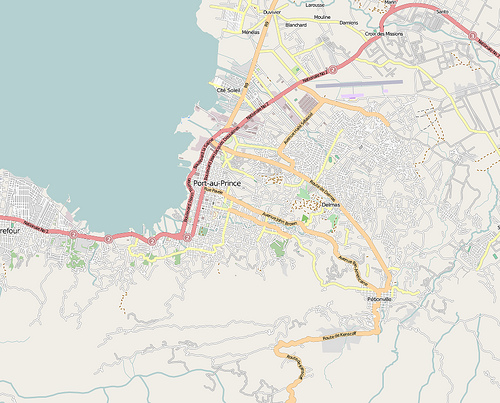
\includegraphics[scale=0.6]{OpenStreetMap/haiti_dopo.jpg}
	\caption{Mappa OSM di Pourt-au-Prince 48 ore dopo il terremoto del 2010}
	\label{fig: haiti_day2}
\end{figure}

La mappa nelle settimane successive continuò ad essere aggiornata e raffinata, tutto questo ha facilitato il coordinamento delle operazioni umanitarie di soccorso e approvigionamento, salvando di fatto innumerevoli vite.\\
In conclusione OSM garantisce un'ottima scalabilità, caratteristica che come abbiamo visto, nei contesti di disaster-management è di fondamentale importanza. 